

\textbf{wir untersuchen das System mit den Parametern T1 Tt}
\textbf{Eingabe des Systems in Computer Algebra (syms)}

\textbf{Eingabe des Systems in Matlab}
\section{Vorgehen in Regelungstechnik}
Zur Ermöglichung einer strukturierten Vorgehensweise bedarf es einer Orientierung. Dieser Arbeit liegt die in der Vorlesung behandelte Vorgehensweise in der Regelungstechnik zugrunde, welche nachfolgend erläutert wird.

\begin{enumerate}
    \item Detaillierungsgrad für das System festlegen
    \item Physikalisches Modell einschließlich der Störsignale erstellen
    \item Eingangs-, Ausgangs-, Zustands- und Störgrößen des Systems festlegen
    \item Physikalische Einheiten festlegen und ggf. Normierung in Prozent
    \item Analyse des Modells
    \begin{enumerate}
        \item Ruhelagen, Anfangswerte, evtl. Linearisierung nichtlinearer Systeme
        \item Systemeigenschaften ermitteln
    \end{enumerate}
    \item Entwurf
    \begin{enumerate}
        \item Ziele, Arbeitspunkte und Trajektorien festlegen
        \item Entwurf: Struktur, Bereich, Verfahren und Kriterien
    \end{enumerate}
    \item Simulation und Rückinterpretation
\end{enumerate}

\section{Das System}


\subsection{Eigenschaften des Systems}

Folgend eine Liste der Eigenschaften des Systems, die sich aus der Übertragungsfunktion $G(s)$ ergibt:

\begin{itemize}
    \item Nennergrad - Zählergrad = 1, dadruch ist das System nicht sprungfähig, antwortet aber sofort mit einer Steigung. Außerdem ist die $D-Matrix$ (welche einem Sprung am Anfang ensprechen würde) $0$.
    \item Ein $PT_3$-Glieder
    \item P-Verhalten mit positiver Verstärkung
    \item gerade Anzahl nicht-minimalphasige rechtsseitiger Nullstellen: Dadurch antwortet das System erst falsch
    \item es gibt 3 reelle negative Polstellen, somit ist das System stabil
\end{itemize}

\subsection{Die Übertragungsfunktion}

Formel \ref{eq:G(s)_1} zeigt die Übertragungsfunktion die in diesem Skript analysiert wird. Formel \ref{eq:G(s)_3} zeigt dann die ausmultiplizierte Formel, sodass die Eigenschaften des Systems leichter zu lesen sind.

\begin{eqnarray}
    \label{eq:G(s)_1}
    G(s) &=& \frac{Y(s)}{U(s)} \\
    \label{eq:G(s)_2}
    &=& \frac{(1-2s)(1-3s)}{(1+4s)(1+5s)(1+6s)} \\
    \label{eq:G(s)_3}
    &=& \frac{6s^2 - 5s + 1}{120s^3 + 74s^2 + 15s +1}
\end{eqnarray}

\section{Darstellungsformen des Systems}

\subsection{Explizite Darstellung des Übertragungsoperators}

\subsection{Eingangs-Ausgang Differentialgleichung}

\begin{eqnarray*}
    G(s) =\frac{Y(s)}{U(s)} &=& \frac{6s^2 - 5s + 1}{120s^3 + 74s^2 + 15s +1} \\
    Y(s)(120s^3 + 74s^2 + 15s +1) &=& U(s) (6s^2 - 5s + 1) \\
    120 \dddot y + 74 \ddot y + 15 \dot y &=& 6 \ddot u + 5 \dot u + u
\end{eqnarray*}

\subsection{Zustandsraumdarstellung}
Das soll man iwie unter 2b einordnen?

Die allgemeine Form der Zustandsraumdarstellung lautet:

\begin{align*}
    \dot x & = Ax + Bu \nonumber \\
    y & = Cx + Du
\end{align*}

Für unser System sieht dies folgendermaßen aus:


\begin{subequations}
    \begin{align}
        \dot x & = \begin{bmatrix}
            -1
        \end{bmatrix}x + \begin{bmatrix}
            2
        \end{bmatrix}u \\
        y & = \begin{bmatrix}
            1.5
        \end{bmatrix}x + \begin{bmatrix}
            0
        \end{bmatrix}u
    \end{align}
\end{subequations}

Man kann auch die Zustandsraumdarstellung direkt eingeben, indem man man die Matrizen $A, B, C, D$ belegt und den Befehl \texttt{sys = ss(A, B, C, D)} ausführt. Von hier aus kommt man mit \texttt{tf(sys)} wieder zur Übertragungsfunktion.

Die Zustandsraumdarstellung kann aus der Übertragungsfunktion in einfachen Fällen mit dem Substitutionstrick erstellt werden. Für Systeme, bei denen auch $\dot u, \ddot u, \ldots$ vorkommt, ist das Ganze ein bisschen komplizierter, wird aber in \href{https://de.wikipedia.org/wiki/Zustandsraumdarstellung#Regelungsnormalform}{Wikipedia} beschrieben und kann entsprechend angewendet werden.
Bei sprungfähigen Systemen sieht das noch etwas anders aus und es muss erst eine Polynomdivision gemacht werden, um $d$ zu erhalten. Im Mehrgrößenfall ist es noch komplizierter. (Weiß Hr. Groell auch nicht)

ACHTUNG: Beim Erstellen dieses Dokuments hatte ich zuerst die ANfangswerte vergessen! Das passiert mir in der Klausur nicht, da sonst ein Punkt weg ist !AUSRUFEZEICHEN!11!!1!
Die Anfangswerte werden für die Simulation natürlich benötigt, weil die Funktion wissen muss, wo sie startet.
Die Anfangswerte müssen mit den Anfangswerten der Ein-  Ausgangsdarstellung korrespondieren. 
Das bedeutet $y(0) = CX(0^-) + D(0^-)$

$ \dot y(0^-) = CAx(0^-) + CBu(0^-) + D \dot u (0^-)$
















\subsubsection{Originale Zustandsraumdarstellung}

Dabei ist eine Möglichkeit Variante in der Zustandsraumdarstellung das zu behandelnde System zu beschreiben die Folgende:

\begin{eqnarray*}
    \dot x &=& \left(\begin{array}{ccc} -0.6167 & -0.25 & -0.1333\\ 0.5 & 0 & 0\\ 0 & 0.125 & 0 \end{array}\right) x + \left(\begin{array}{c} 0.5\\ 0\\ 0 \end{array}\right) u  \nonumber \\
    y &=& \left(\begin{array}{ccc} 0.1 & -0.1667 & 0.2667 \end{array}\right) x
\end{eqnarray*}

\subsubsection{Ähnlichkeitstransformation}

Durch eine Ähnlichkeitstransformation können mit der Hilfmatrix $T$ in \ref{eq:T} folgenden Matrizen in der Zustandsraumdarstellung erzeugt werden.

\begin{equation*}
    \label{eq:T}
    T = \left(\begin{array}{ccc} 1 & 2 & 3\\ 0 & 1 & 3\\ 9 & 0 & 1 \end{array}\right)
\end{equation*} 

\begin{eqnarray*}
    \dot x &=& \left(\begin{array}{ccc} 0.1771 & -0.2292 & 0.02292\\ 0.3795 & -0.3839 & 0.01339\\ -1.862 & 1.598 & -0.4098 \end{array}\right)x + \left(\begin{array}{c} 0.5\\ 0\\ 4.5 \end{array}\right)u \\
    y &=& \left(\begin{array}{ccc} -0.2429 & 0.319 & 0.0381 \end{array}\right)x
\end{eqnarray*}



\section{Simulation des Systems}

\subsection{Sprungantwort}

In Abbildung \ref{fig:sprung} ist die Reaktion des Systems auf den Heaviside-Funktion zu sehen. Diese ist wie folgt definiert:

\[
\sigma (t) = \begin{cases} 0 & \text{für t < 0} \\ 1 & \text{für t > 0} \end{cases}  
\]

\begin{figure}[H]
    \label{fig:sprung}
    \centering
    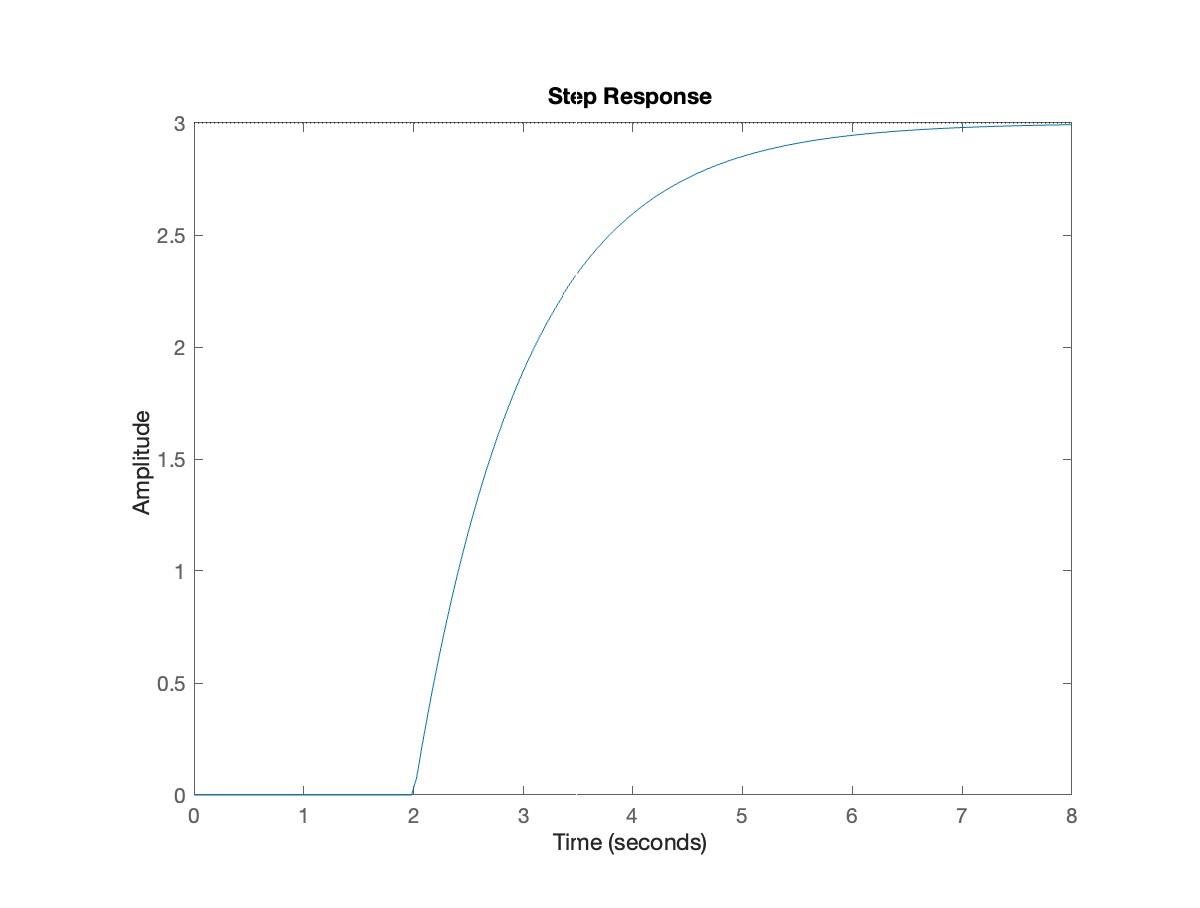
\includegraphics[width=0.8\textwidth]{Bilder/SprungantwortPT1Tt.eps}
    \caption{Sprungantwort}
 \end{figure}


\subsection{Impulsantwort}

In Abbildung \ref{fig:impuls} ist die Reaktion des Systems auf den Dirac-Funktion zu sehen. Die Dirac-Funktion ist die Ableitung der Heaviside-Funktion und definiert durch:

\[
    \delta (t) \stackrel{D'}{=} \frac{d}{dt} \sigma (t)
\]

Die wichtigste Eigenschaft der Dirac-Funktion ist, dass die Fläche unter dem Impuls exakt $1$ ist. Daraus folgt:

\[
    \int_{-\infty}^\infty \delta (t) dx = 1
\]

\begin{figure}[H]
    \label{fig:impuls}
    \centering
    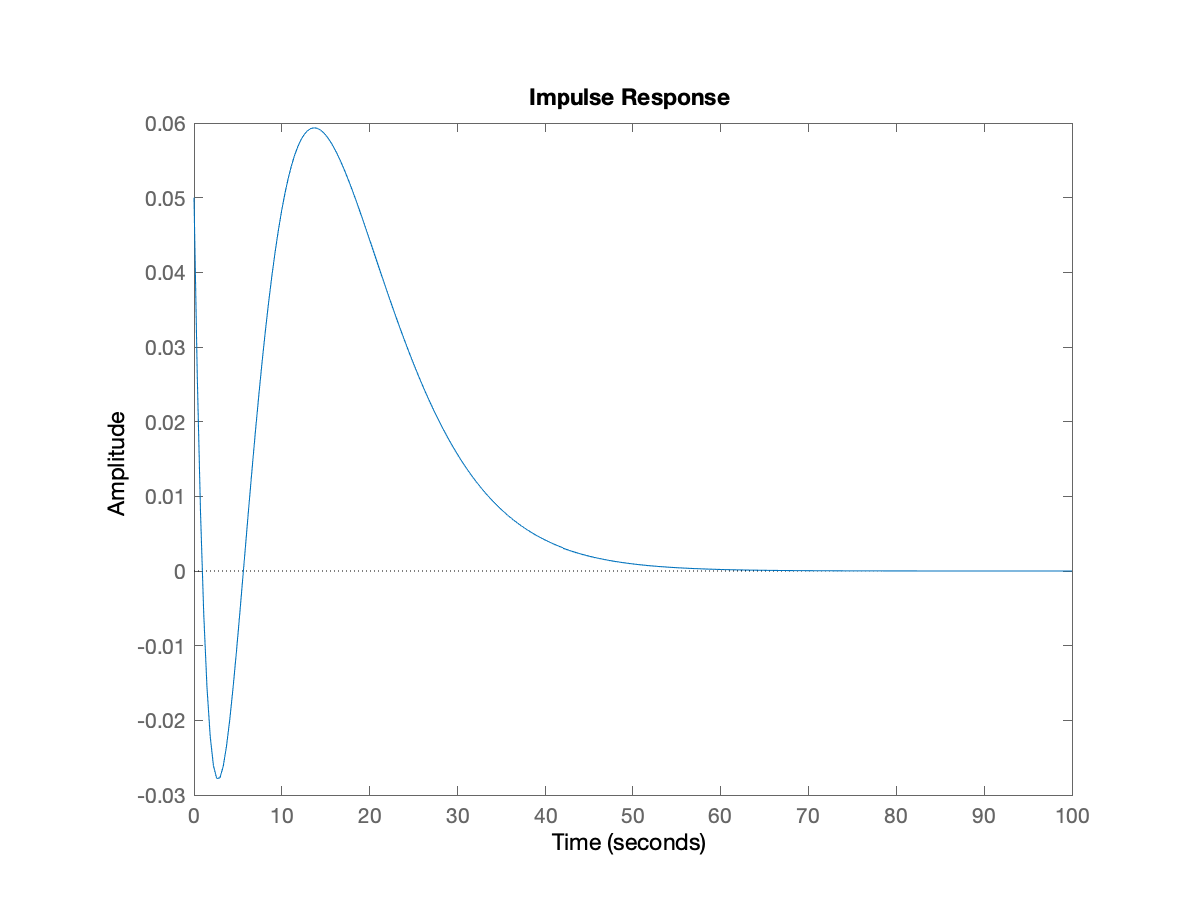
\includegraphics[width=0.8\textwidth]{Bilder/ImpulsAntwort.eps}
    \caption{Impulsantwort}
\end{figure}

\subsection{explizite Lösung}

Durch die inverse Laplacetransformation lässt sich die explizite Lösung des Systems für die Impulsfunktion als Eingangssignal ermitteln.

\[
    L^{-1}\{\frac{6s^2 - 5s + 1}{120s^3 + 74s^2 + 15s +1}\} = \frac{21\,{\mathrm{e}}^{-\frac{t}{4}}}{4}-\frac{56\,{\mathrm{e}}^{-\frac{t}{5}}}{5}+6\,{\mathrm{e}}^{-\frac{t}{6}}
\]


\subsection{statischer Verstärkungsfaktor}

Wie in Abbildung \ref{fig:sprung} zu sehen pendelt sich der Ausgang des System bei $1$ ein. Das passiert, weil $ k = 1$ ist.
Ein Graph des Verstärkungsfaktor, wobei auf der $x-Achse$ die konstanten Eingänge und auf der $y-Achse$ die Ausgänge des Systems für $t \rightarrow \infty$.

\begin{figure}[H]
    \label{fig:Kennline}
    \centering
    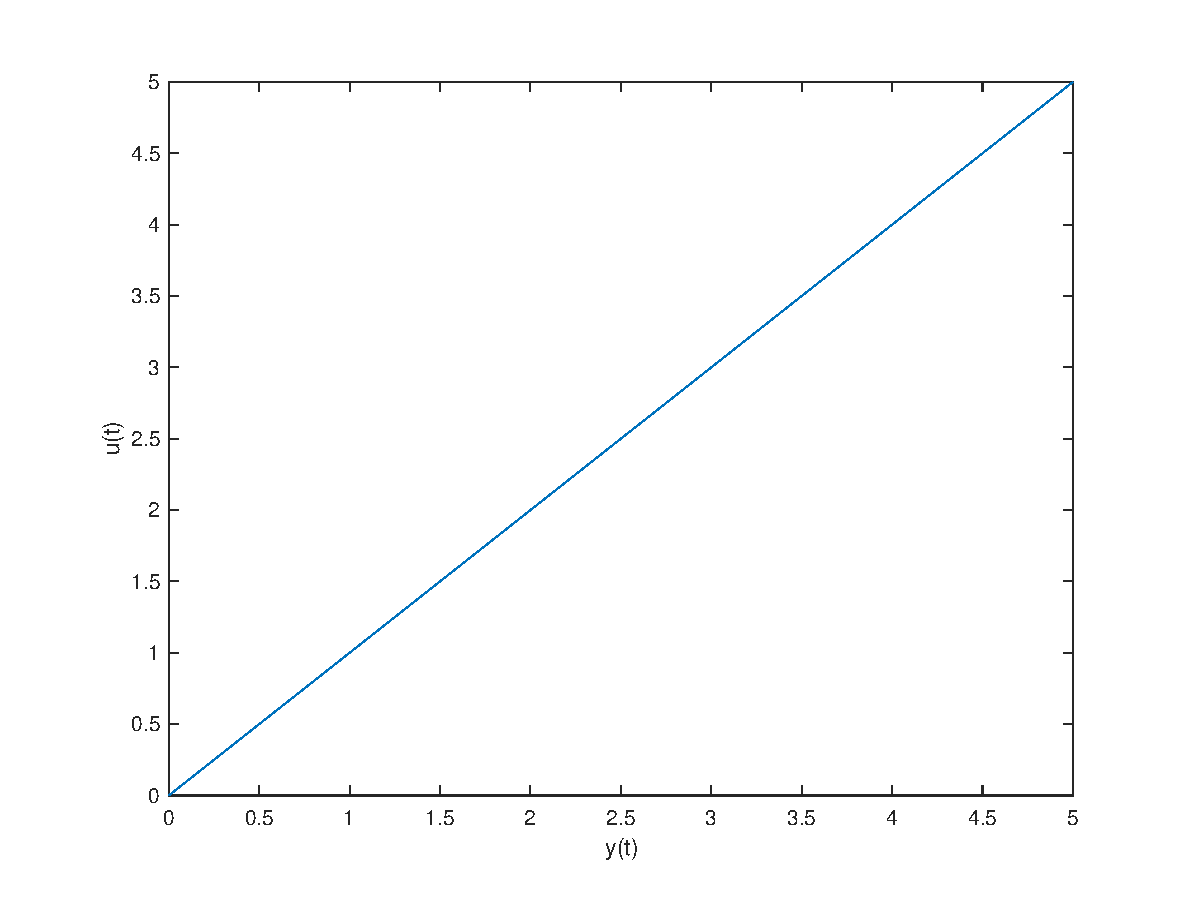
\includegraphics[width=0.5\textwidth]{Bilder/Kennlinie.eps}
    \caption{statischer Verstärkungsfaktor}
\end{figure}


\section{Verhalten bei Schwingungseingängen}

\subsection{Nullstellen und Pole}

Abbildung \ref{fig:pzmap} zeigt einen Pole-Zero-Plot zu dem System, welcher als \textbf{x} markiert die Nullstellen des Systems und mit \textbf{o} markiert die Polstellen des System zeigt.

Das System hat 3 Polstellen auf der reellen Achse in der linken Halbebene, was ebenfalls die Stabilität des Systems zeigt, und 2 nicht-minimalphasige Nullstellen auf der reellen Achse, also in der rechten Halbebene.

\begin{figure}[H]
    \label{fig:pzmap}
    \centering
    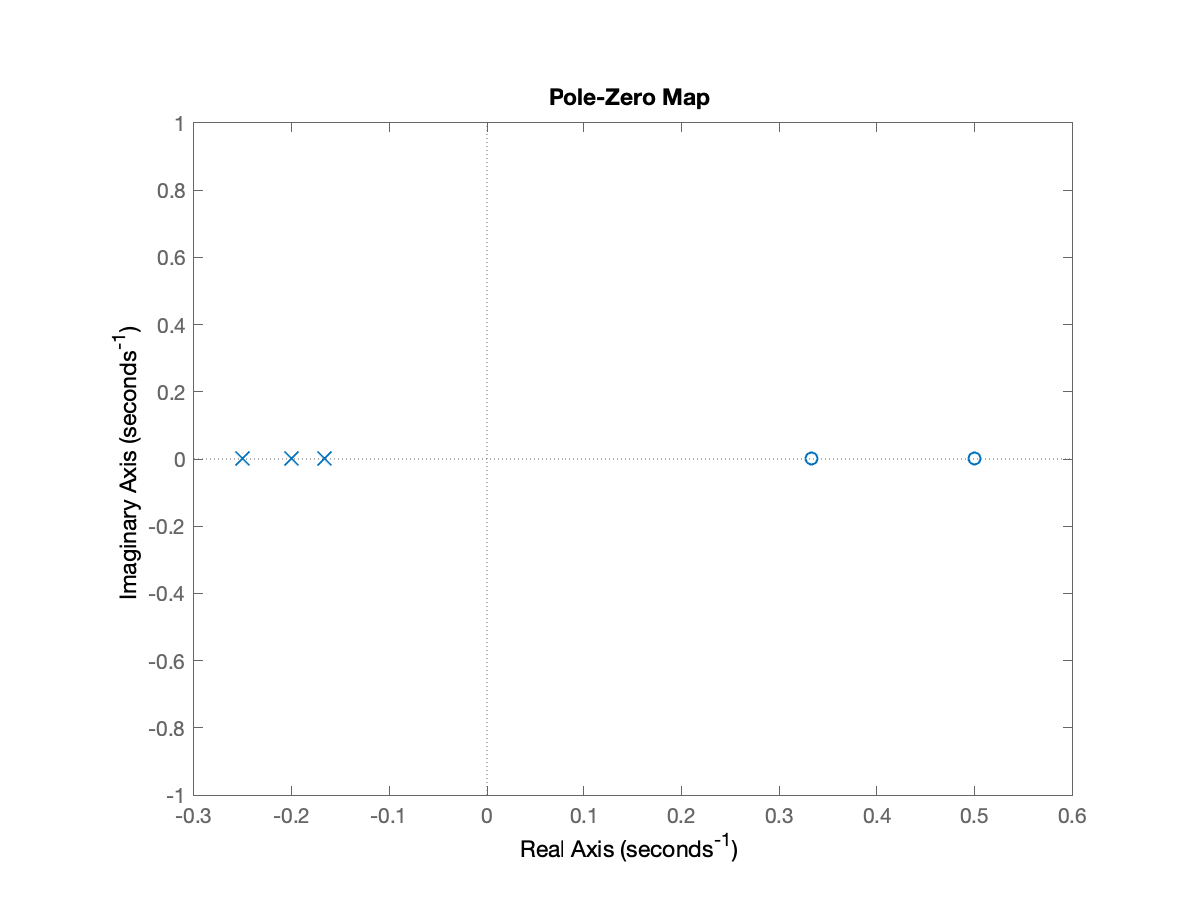
\includegraphics[width=0.8\textwidth]{Bilder/PoleZeroPlot.eps}
    \caption{Pole-Zero-Plot}
 \end{figure}


\subsection{Bode-Plot}

In Abbildung \ref{fig:bode} ist die Amplitude und die Phase des Systemausgangs in Abhängigkeit zur Frequenz (logarithmisch skaliert).

\begin{figure}[H]
    \label{fig:bode}
    \centering
    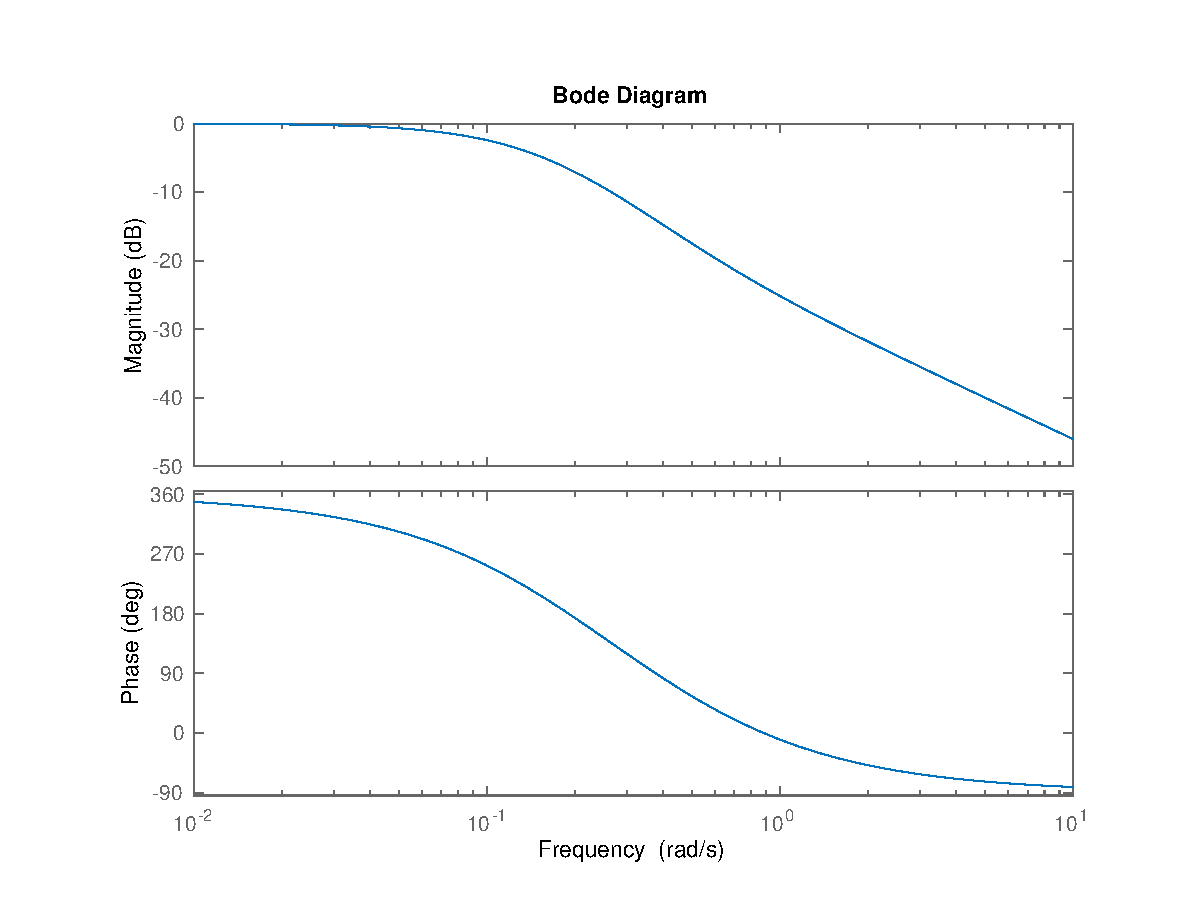
\includegraphics[width=0.8\textwidth]{Bilder/Bode.eps}
    \caption{Bode-Plot}
 \end{figure}

\subsection{Nyquist-Plot}

Die Ortskurve oder auch Nyquist-Plot in \ref{fig:nyquist} ist ein Graph der die Amplitude und Phase des Systems für Schwingungen mit allen Frequenzen darstellt.

\begin{figure}[H]
    \label{fig:nyquist}
    \centering
    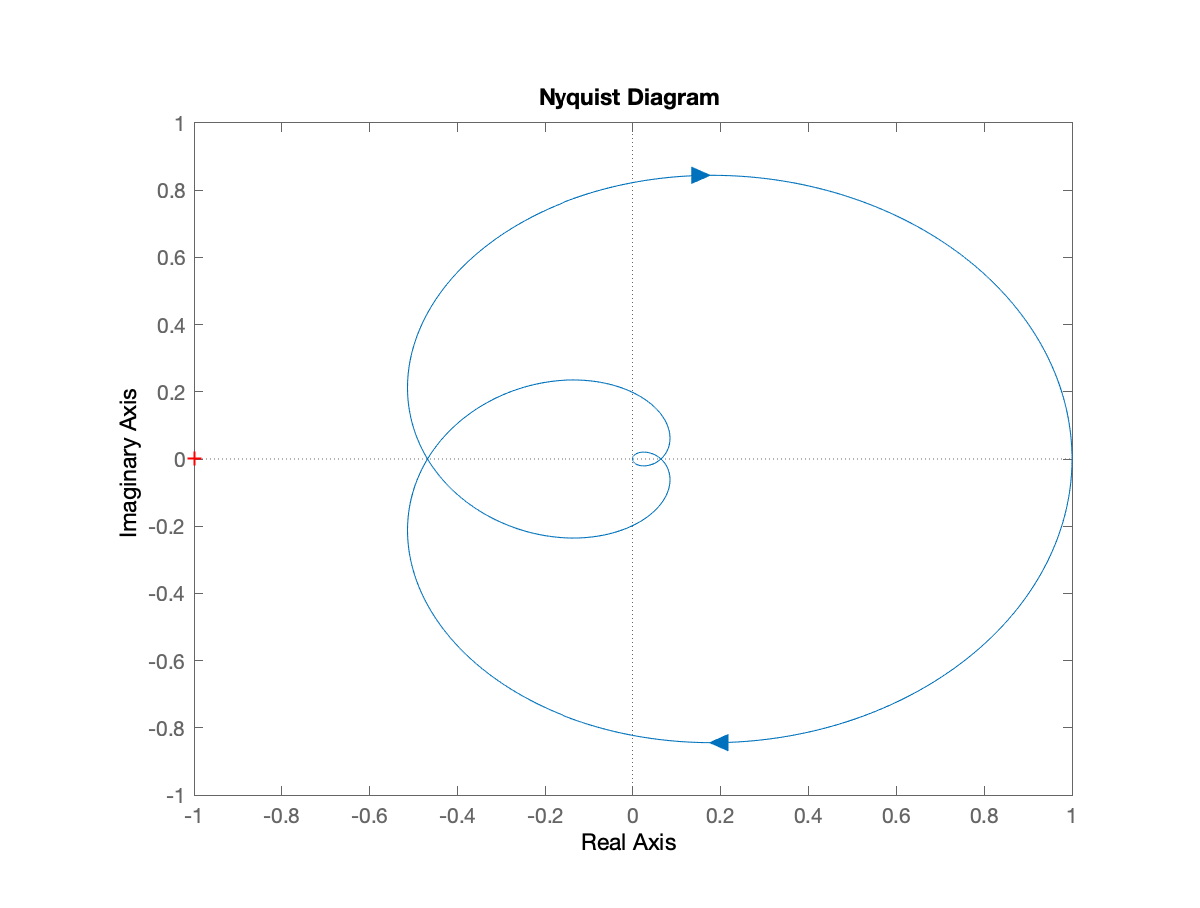
\includegraphics[width=0.8\textwidth]{Bilder/Nyquist.eps}
    \caption{Ortskurve / Nyquist-Plot}
 \end{figure}